% !TEX program = XeLaTeX
% !TEX encoding = UTF-8
\documentclass[UTF8,nofonts]{article}
%{ctexart}


%\setCJKmainfont[BoldFont=FandolSong-Bold.otf,ItalicFont=FandolKai-Regular.otf]{FandolSong-Regular.otf}
%\setCJKsansfont[BoldFont=FandolHei-Bold.otf]{FandolHei-Regular.otf}
%\setCJKmonofont{FandolFang-Regular.otf}

\usepackage{url}
\usepackage{cancel}
\usepackage{xspace}
\usepackage{graphicx}
\usepackage{multicol}
\usepackage{multirow}
\usepackage{subfig}
\usepackage{amsmath}
\usepackage{amssymb}
\usepackage[a4paper, width=186mm, top=18mm, bottom=18mm, includeheadfoot]{geometry}
%\usepackage[a4paper, width=140mm, top=18mm, bottom=22mm, includeheadfoot]{geometry}
\usepackage{booktabs}
\usepackage{array}
\usepackage{verbatim}
\usepackage{caption}
\usepackage{natbib}
\usepackage{booktabs}
\usepackage{float}
\usepackage{pdflscape}
\usepackage{mathtools}
\usepackage[usenames, dvipsnames]{xcolor}
\usepackage{afterpage}
\usepackage{pgf}
\usepackage{tikz}
\usepackage{dirtree}
\usepackage{amsfonts}
\usepackage{tikz}
\usepackage{tkz-graph}
\usetikzlibrary{arrows,decorations.pathmorphing,automata,positioning,backgrounds,fit,shapes.symbols,chains,intersections}

\newtheorem{definition}{Definition}[section]
\newtheorem{theorem}{Theorem}[section]
\newtheorem{lemma}{Lemma}
\newtheorem{proof}{Proof} [section]



\usepackage[toc, page, title, titletoc, header]{appendix}
\usepackage{marginnote}
\usepackage{tablefootnote}

%\renewcommand\appendixname{附\ 录}
%\renewcommand\appendixpagename{附\ 录}
%\renewcommand\appendixtocname{附\ 录}
\renewcommand\abstractname{Abstract}


\usepackage{perpage} %the perpage package
\MakePerPage{footnote} %the perpage package command

\usetikzlibrary{shapes.geometric}%
\usepackage{color}
%\usepackage[pages=some, placement=top]{background}
\usepackage{eso-pic}
\usepackage[final]{pdfpages}

%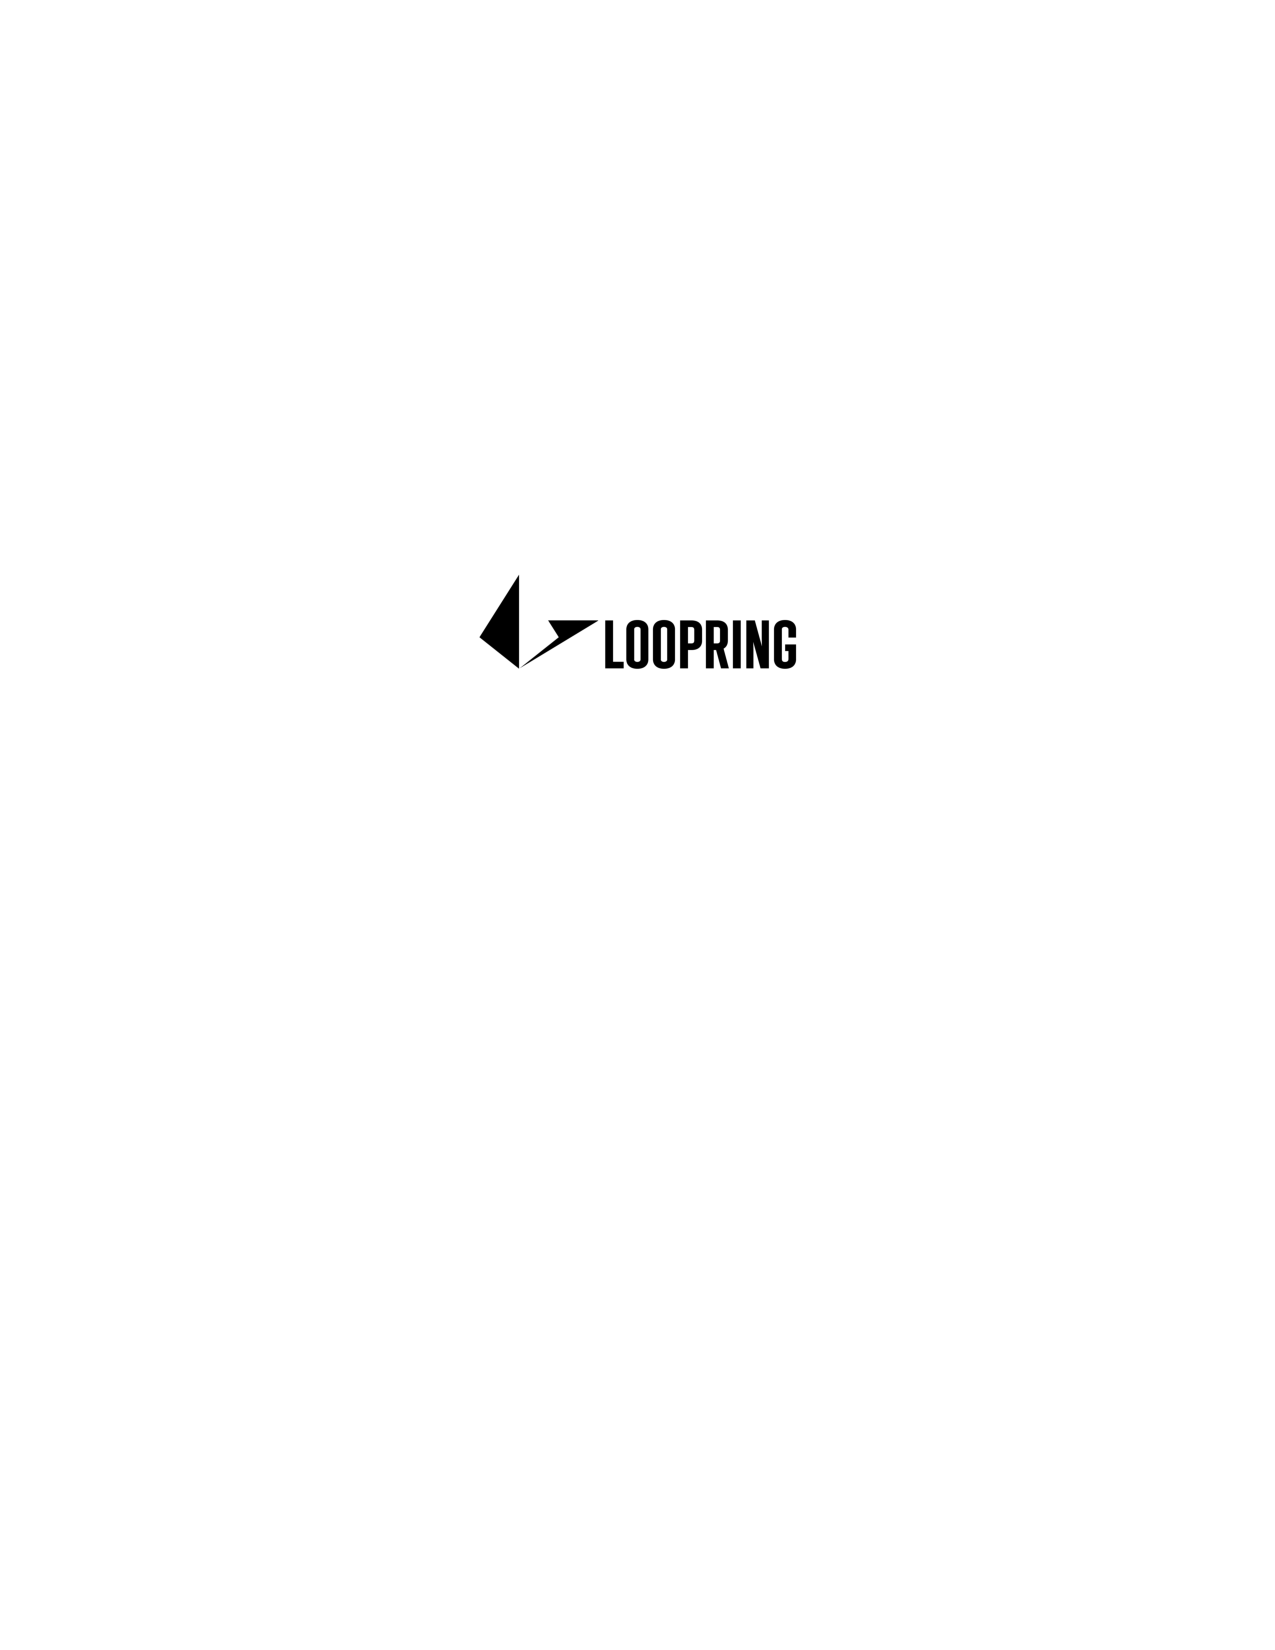
\includepdf[pages=1]{cover}
\hyphenpenalty=750

\title{\textbf{Loopring:}\\\textbf{A Decentralized Token Exchange Protocol}}
\author{
  Daniel Wang\\
  \texttt{daniel@loopring.org}\\
  \and
  	Jay Zhou\\
  	\texttt{jay@loopring.org}\\
  	\and
  	Alex Wang\\
  	\texttt{alex@loopring.org}\\
  	\and
  	Matthew Finestone\\
  	\texttt{matt.finestone@gmail.com}\\ 
  \\
  \texttt{https://loopring.org}
 }

\makeatletter
\def\CTEX@section@format{\Large\bfseries}
\makeatother

\makeatletter
\newenvironment{tablehere}
 {\def\@captype{table}}
 {}

\newenvironment{figurehere}
 {\def\@captype{figure}}
 {}
\makeatother
%
%\newcommand\BackgroundPic{%
%\put(0, 0){%
%\parbox[b][\paperheight]{\paperwidth}{%
%\vfill
%\centering
%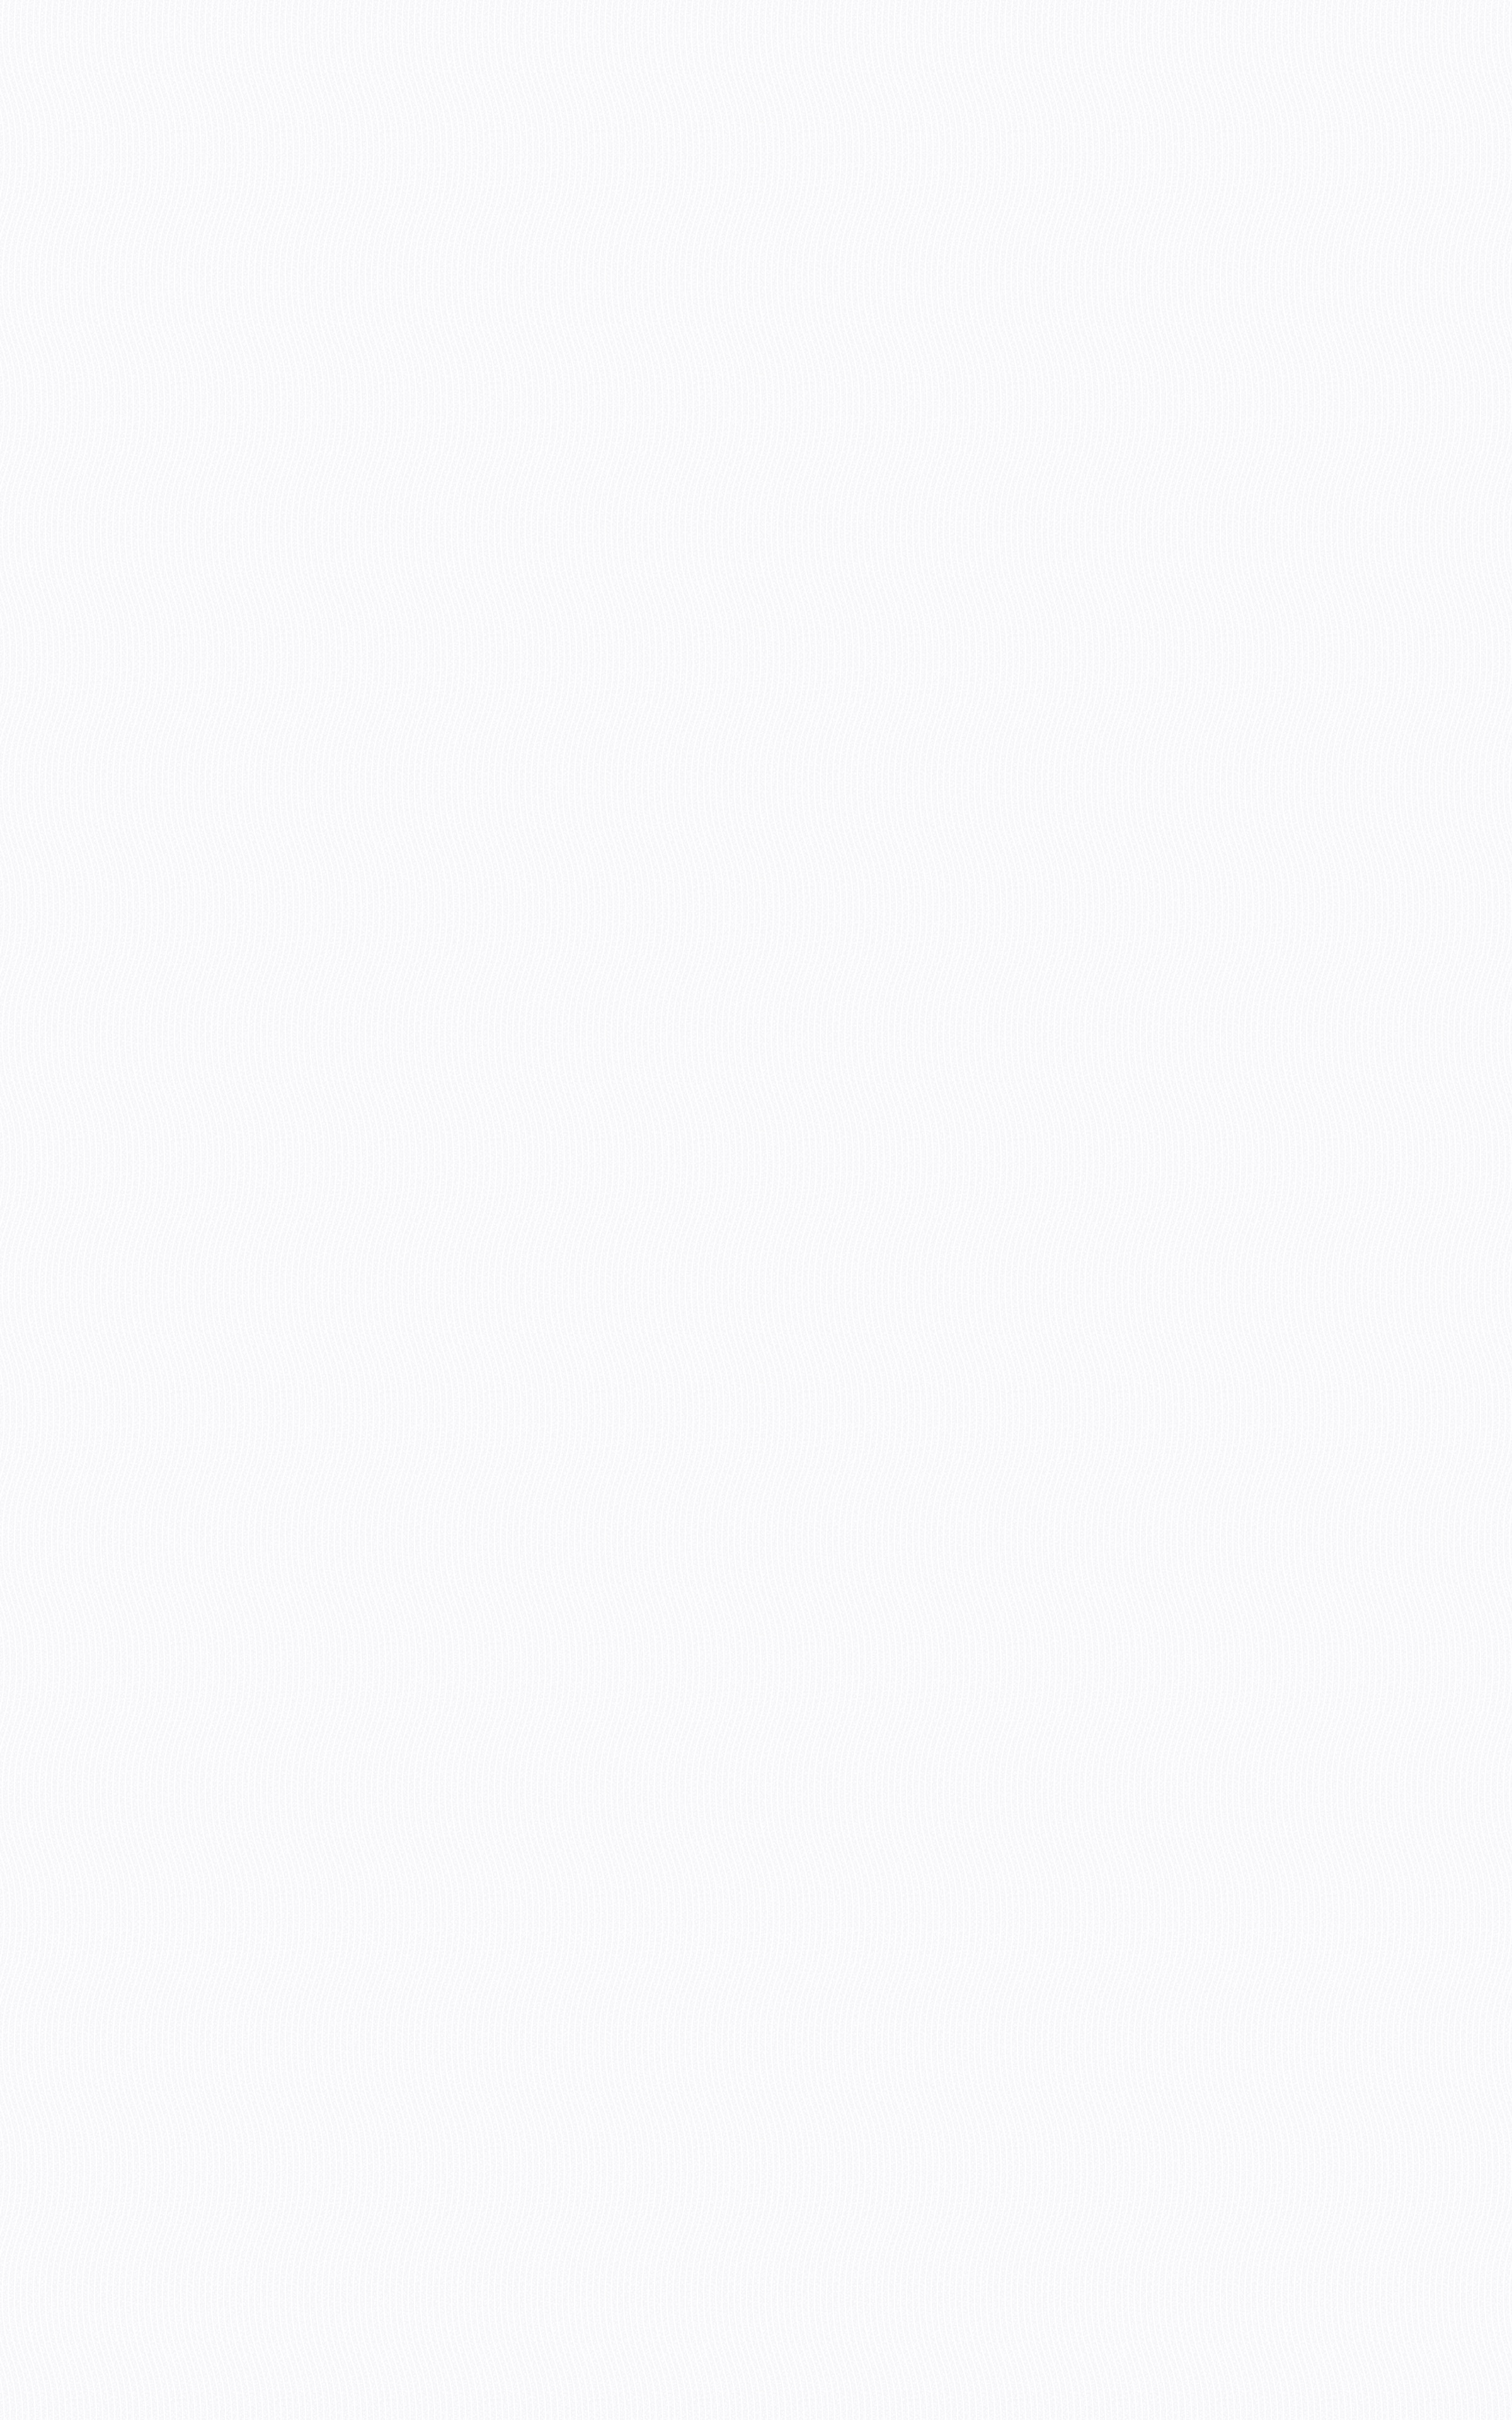
\includegraphics[width=\paperwidth, height=\paperheight, %
%%keepaspectratio]{images/background.jpg}%
%]{images/background.jpg}%
%\vfill
%}}}


\begin{document}
%\AddToShipoutPicture{\BackgroundPic}
\maketitle


\begin{abstract}
Loopring is an open protocol for building decentralized exchanges. Loopring operates as a public set of smart contracts responsible for trade and settlement, with an off-chain group of actors aggregating and communicating orders. The protocol is free, extensible, and serves as a standardized building block for decentralized applications (dApps) that incorporate exchange functionality. Important improvements over current decentralized exchange protocols include the ability for users' orders to be mix-and-matched with other orders, obviating the constraints of two-token trading pairs, drastically improving liquidity, and allowing for price improvement possibility. Loopring also employs a robust and unique solution to prevent front-running: the unfair attempt to submit transactions into a block quicker than the original solution provider. Loopring is blockchain agnostic, and deployable on any blockchain with smart contract functionality. At the time of writing, it's operable on Ethereum \cite{buterin2017ethereum} \cite{wood2014ethereum} and Qtum \cite{dai2017smart} with NEO \cite{atterlonn2018distributed} also under construction. Its interoperable standards ensure trustless, decentralized, and anonymous trading.
\end{abstract}



\begin{multicols}{2}
\section{Introduction\label{sec:introduction}}

With the proliferation of blockchain-based assets, the need to exchange these assets amongst counterparties has significantly increased. As thousands of new tokens are introduced - including the tokenization of traditional assets - this need is magnified. Whether exchanging tokens for speculative trading motivations, or converting to access networks via their native utility tokens, the ability to exchange one cryptoasset for another is foundational for the larger ecosystem. Indeed, there is a potential energy in assets \cite{desotocapital}, and realizing this energy - unlocking capital - requires not only asserting ownership, which blockchains have allowed for with immutability,  but the ability to freely transfer and transform these assets.
 
As such, the trustless exchange of tokens (value) is a compelling use case for blockchain technology. Until now, however, crypto enthusiasts have largely settled for trading tokens on traditional centralized exchanges. The Loopring protocol is needed because, just as Bitcoin \cite{nakamoto2008bitcoin} dutifully pointed out that, in regards to peer-to-peer electronic cash, "the main benefits are lost if a trusted third party is still required to prevent double-spending", so too are the main benefits of decentralized assets lost if they must pass through trusted, gated, centralized exchanges.

Trading decentralized tokens on centralized exchanges doesn't make sense from a philosophical perspective, as it fails to uphold the virtues these decentralized projects espouse. There are also numerous practical risks and limitations in using centralized exchanges which are described below. Decentralized exchanges (DEXs) \cite{schuh2015bitshares} \cite{bancor} \cite{kyber} have sought to address these issues, and in many cases have succeeded in alleviating security risks by using blockchains for disintermediation. However, as DEX capability becomes important infrastructure for the new economy, there is substantial room for improvement in performance. Loopring aims to provide critical tools for said infrastructure with its dApp agnostic open protocol. 

\section{Current Exchange Landscape\label{sec:current_exchange_landscape}}

\subsection{Inadequacies of Centralized Exchanges}
The three primary risks of centralized exchanges are; 1) Lack of security, 2) Lack of transparency, and 3) Lack of liquidity.

\textbf{Lack of Security} arises from users typically surrendering control of their private keys (funds) to one centralized entity. This exposes users to the possibility that centralized exchanges fall prey to malicious hackers. The security and hacking risks facing all centralized exchanges are well known \cite{coincheckhack} \cite{mtgox} \cite{mcmillan2014inside}, yet are often accepted as "table stakes" for token trading. Centralized exchanges continue to be honeypots for hackers to attack as their servers have custody over millions of dollars of users' funds. Exchange developers can also make honest, accidental errors with user funds. Users are simply not in control of their own tokens when deposited at a centralized exchange.

\textbf{Lack of Transparency} exposes users to the risk of dishonest exchanges acting unfairly. The distinction here is by the exchange operator's malintentions since users are not truly trading their own assets on a centralized exchange, but rather, an IOU. When tokens are sent to the exchange's wallet, the exchange takes custody, and offers an IOU in its place. All trades are then effectively between users' IOUs. To withdraw, users redeem their IOU with the exchange, and receive their tokens to their external wallet address. Throughout this process there is a lack of transparency, and the exchange can shutdown, freeze your account, go bankrupt, etc. It is also possible that they use user assets for other purposes while in custody, such as lending them out to third parties. Lack of transparency can cost users without a total loss of funds, such as in higher trading fees, delays at peak demand, regulatory risk, and orders being front ran.

\textbf{Lack of Liquidity.} From the point of view of exchange operators, fragmented liquidity inhibits entry by new exchanges because of two winner-takes-all scenarios. First, the exchange with the greatest number of available trading pairs wins, because users find it desirable to conduct all their trades on one exchange. Second, the exchange with the largest order book wins, because of favorable bid-ask spreads for each trading pair. This discourages competition from newcomers because it is difficult for them to build up initial liquidity. As a result, many exchanges command a high market share despite user complaints and even major hacking incidents. It's worth noting that as centralized exchanges win market share, they become an ever-larger hacking target. 

From the point of view of users, fragmented liquidity significantly reduces user experience. In a centralized exchange, users are only able to trade within the exchange's own liquidity pools, against its own order book, and between its supported token pairs. To trade Token A for Token B, users must go to an exchange that supports both tokens or register at different exchanges, disclosing personal information. Users often need to execute preliminary or intermediate trades, typically against BTC or ETH, paying bid-ask spreads in the process. Finally, the order books may not be deep enough to complete the trade without material slippage. Even if the exchange purports to process large volumes, there is no guarantee that this volume and liquidity is not fake \cite{fakevolume}.

The result is disconnected silos of liquidity and a fragmented ecosystem that resembles the legacy financial system, with significant trading volume centralized on few exchanges. The global liquidity promises of blockchains hold no merit within centralized exchanges.

\subsection{Inadequacies of Decentralized Exchanges}
Decentralized exchanges differ from centralized exchanges in part because users maintain control of their private keys (assets) by performing trades directly on the underlying blockchain. By leveraging the trustless technology of cryptocurrencies themselves, they successfully mitigate many of the abovementioned risks surrounding security. However, problems persist in regards to performance and structural limitations. 

Liquidity often remains an issue as users must search for counterparties across disparate liquidity pools and standards. Fragmented liquidity effects are present if DEXs or dApps at large don't employ consistent standards to interoperate, and if orders are not shared/propagated across a wide network. The liquidity of limit order books, and, specifically, their resiliency - how fast filled limit orders are regenerated - can significantly affect optimal trading strategies \cite{limitorderliquidity}. The absence of such standards has resulted not only in reduced liquidity, but also exposure to an array of potentially insecure proprietary smart contracts.

Furthermore, since trades are performed on chain, DEXs inherit the limitations of the underlying blockchain, namely: scalability, delays in execution (mining), and costly modifications to orders. Thus, blockchain order books do not scale particularly well, as executing code on the blockchain incurs a cost (gas), making multiple order-cancel cadences prohibitively expensive. 

Finally, because blockchain order books are public, the transaction to place an order is visible by miners as it awaits being mined into the next block, and placed into an order book. This delay exposes the user to the risk of being front run and having the price or execution move against him.

\subsection{Hybrid Solutions}
For the above reasons, purely blockchain-based exchanges have limitations that make them uncompetitive with centralized exchanges. There is a tradeoff between on-chain inherent trustlessness, and centralized exchange speed and order flexibility. Protocols such as Loopring and 0x \cite{warren20170x} extend a solution of on-chain settlement with off-chain order management. These solutions revolve around open smart contracts, but navigate scalability limitations by performing several functions off-chain and giving nodes flexibility in fulfilling critical roles for the network. However, drawbacks remain for the hybrid model as well \cite{costofdecent}. The Loopring protocol proposes meaningful differences in our approach to a hybrid solution throughout this paper.


\section{Loopring Protocol\label{sec:loopring_protocol}}
Loopring is not a DEX, but a modular protocol for building DEXs on multiple blockchains. We disassemble the component parts of a traditional exchange and offer a set of public smart contracts and decentralized actors in its place. The roles in the network include wallets, relays, liquidity-sharing consortium blockchains, order book browsers, ring-miners, and asset tokenization services. Before defining each, however, we should first understand what a Loopring compliant order looks like. 

\subsection{Order Ring\label{sec:order_ring}}
Loopring orders are expressed in what we call a Unidirectional Order Model (UDOM \cite{coinport2014udom}). UDOM expresses orders as token exchange requests, $amountS \over amountB$, (amount to sell/buy)  instead of bids and asks. Since every order is just an exchange rate between two tokens, a powerful feature of the protocol is the mixing and matching of multiple orders in circular trade. By using up to 10 orders instead of a single trading pair, there is a dramatic increase in liquidity and potential for price improvement. 

\begin{center}
\begin{figurehere}
\centering
\tikzstyle{block} = [draw, fill=blue!20, rectangle, 
    minimum height=3em, minimum width=6em]
\tikzstyle{sum} = [draw, fill=blue!20, circle, node distance=1cm]
\tikzstyle{input} = [coordinate]
\tikzstyle{output} = [coordinate]
\tikzstyle{pinstyle} = [pin edge={to-,thin,black}]

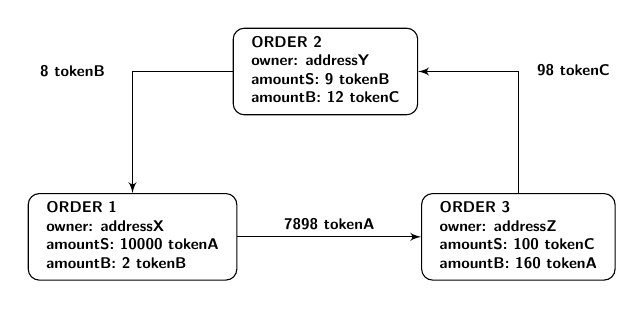
\begin{tikzpicture}[
    auto, 
    node distance=3cm,
    >=latex',
    font=\bfseries\footnotesize\sffamily,
    order/.style={
		scale=0.7,
		rectangle,
		rounded corners,
		draw=black, 
		text centered,
%		text width=5cm,
		minimum height=12mm,
		fill=white
	},
	label/.style={
		scale=0.7
	}
  ]
    % We start by placing the blocks

  \node [order] (order2) 
 {%
 \begin{tabular}{l}
  \textbf{ORDER 2}\\
  \textbf{owner: addressY}\\
  \textbf{amountS: 9  tokenB}\\
  \textbf{amountB: 12 tokenC}
 \end{tabular}
 };
 
  \node [order, below of=order2, xshift=-3.5cm] (order1) 
 {%
 \begin{tabular}{l}
  \textbf{ORDER 1}\\
  \textbf{owner: addressX}\\
  \textbf{amountS: 10000 tokenA}\\
  \textbf{amountB: 2    tokenB}
 \end{tabular}
 };
 
 
  \node [order, below of=order2, xshift=3.5cm] (order3) 
 {%
 \begin{tabular}{l}
  \textbf{ORDER 3}\\
  \textbf{owner: addressZ}\\
  \textbf{amountS: 100 tokenC}\\
  \textbf{amountB: 160 tokenA}
 \end{tabular}
 };
 
 \draw [draw,->] (order1) -- node [label] {\textbf{7898 tokenA}} (order3);
 \draw [draw,->] (order2) -| node [label, xshift=-1.8cm] {\textbf{8 tokenB}} (order1);
 \draw [draw,->] (order3) |- node [label, xshift=1cm, yshift=0.24cm] {\textbf{98 tokenC}} (order2);

\end{tikzpicture}

\caption{A Ring of 3 Orders}
\label{fig:ring}
\end{figurehere}
\end{center}


Each order's token to sell is another order's token to buy. It creates a loop that allows each order to exchange their desired tokens without requiring an opposing order for its pair. Traditional order pair trades can, of course, still be executed, in what is essentially a special case of an Order Ring. 

\begin{definition}[Order Ring] Let $C_{0}$, $C_{1}$, $\cdots$, $C_{n-1}$ be $n$ different kinds of token, $O_{0\rightarrow 1}$, $\cdots$, $O_{i\rightarrow i\oplus 1}$, $\cdots$, $O_{n-1 \rightarrow 0}$ be $n$ orders. Those orders can form a ring for trading:
$$O_{0\rightarrow 1} \rightarrow \cdots \rightarrow O_{i\rightarrow i\oplus 1} \rightarrow \cdots \rightarrow O_{n-1\rightarrow 0} \text{, }$$
where $n$ is the length of the ring, and $i\oplus 1 \equiv i+1 \mod n$.
\end{definition}

An order ring is valid when all component transactions can be executed at an exchange rate equal to or better than the original rate specified by the user. To verify ring validity, Loopring protocol smart contracts must receive Order Rings from miners where the product of the original exchange rates of all orders is equal to or greater than 1.

Let's assume Alice and Bob want to trade their tokens A and B. Alice has 15 tokens A and she wants 4 tokens B for them; Bob has 10 tokens B  and he wants 30 tokens A for them.

Who is buying and who is selling? This depends only on the asset we fix to give price quotations. If token A is the reference, then Alice is buying tokens B for ${15 \over 4} = 3.75$ XTA, while Bob is selling 10 tokens B for ${30 \over 10} = 3.00$ XTA. In the case of fixing token B as reference we say that Alice is selling 15 tokens A for ${4\over 15}=0.26666667$ XTB and Bob is buying 10 tokens A for ${10 \over 30}=0.33333334$ XTB. Hence, who's the buyer or seller is arbitrary.

In the first situation Alice is willing to pay a higher price than the price Bob is selling his tokens for, while in the second situation Bob is willing to pay a higher price than the price Alice is selling her tokens for. It is clear that a trade is possible whenever the buyer is willing to pay an equal or higher price than the seller's price.

\begin{equation}
{{15\over 4} \over {30\over 10}} = {15 \over 4} \cdot {10 \over 30} = {150 \over 120} = 1.25 > 1
\end{equation}

Thus, for a set of n orders to be able to be filled, fully or partially, we need to know if the product of each one of the exchange rates as buy orders results in a number greater or equal to 1. If so, all the n orders can be either partially, or totally filled \cite{supersymmetry}.

If we introduce a third counterparty, Charlie, such that  Alice wants to give x1 tokens A and receive y1 tokens B, Bob wants to give x2 tokens B and receive y2 tokens C, and Charlie wants to give x3 tokens C and receive y3 tokens A. The necessary tokens are present, and the trade is possible if,

\begin{equation}
{{x1 \cdot x2 \cdot x3 \over y1 \cdot y2 \cdot y3} \geq 1}
\end{equation}


See section \ref{anatomy} for more details about Loopring's orders.


\section{Ecosystem Participants\label{sec:ecosystem}}
The following ecosystem participants jointly provide all functionalities a centralized exchange has to offer. 

\begin{itemize}

\item \textbf{Wallets}: A common wallet service or interface that gives users access to their tokens and a way to send orders to the Loopring network. Wallets will be incentivized to produce orders by sharing fees with miners (see section \ref{sec:token}). We believe the future of trading will take place within the safe confines of individual user's wallets; connecting these liquidity pools through our protocol is paramount.

\item \textbf{Relays / Ring Miners}: Relays are nodes that form a decentralized network for order propagation. They maintain public order books and trade history and broadcast new orders to other relays via any arbitrary off-chain medium. Ring-mining is a feature of relays. It is computationally heavy and is done completely off-chain. Ring-mining produces Order Rings: rings of between 2 and 10 orders created by stitching together disparate orders. Relays are free in how they choose to communicate with one another. 

\item \textbf{Consortium Liquidity Sharing Blockchain}: A relay-mesh network for order & liquidity sharing. When nodes run Loopring relay software, they are able to join an existing network and share liquidity with other relays over a consortium blockchain. The consortium blockchain we are building as a first implementation has near real time order sharing (blocks mined every 1-2 seconds), and trims old history to allow for faster download by new nodes. Notably, relays need not join this consortium; they can act alone and not share liquidity with others, or, they can start and manage their own liquidity sharing network.

\item \textbf{Loopring Protocol Smart Contracts (LSC)}: A set of public and free smart contracts that checks Order Rings received from miners, does token transfers on behalf of users, incentivizes miners/wallets with fees, and emits events. Relays/order browsers listen to these events to keep their order books and trade history up to date. See appendix \ref{app:protocol_ethereum} for details.

\item \textbf{Asset Tokenization Services}: A bridge between assets that cannot be directly traded on Loopring. They are centralized services run by trustworthy companies or organizations. A user could deposit his assets (real, fiat or tokens from other chains) and get tokens issued. By returning these tokens the user gets back his deposit. Loopring is not a cross-chain exchange protocol, but Asset Tokenization Services make it possible to trade Ethereum ERC20 \cite{ERC20} tokens with physical assets as well as assets on other blockchains. 

\end{itemize}


\section{Exchange Process\label{sec:process}}
\begin{enumerate} 

\item \textbf{Order Initiation \& ERC20 Authorization}: A user wants to exchange X amount of TokenA for Y amount of TokenB. The current rate and order book for this pair can be found on multiple sources provided by relays or other interfaces hooked up to the network, such as order book browsers. The user places an order through a wallet interface. An amount of LRx can be added to the order as a fee for miners; higher LRx fee means a better chance to be processed earlier by miners. The wallet authorizes the LSC to handle X amount of TokenA the user wants to sell, but does not lock the user's tokens, who remains free to move them while the order is being processed.

\item \textbf{Send order to the network}: Once the authorization is made, the order's data is signed with the private key of the sender. Then, the wallet sends the order along with its signature to one or more nodes (relays) in the network.

\item \textbf{Relay broadcast}: On the reception of the order, relays update their public order book and broadcast the order to other relays/ring miners. The protocol doesn't require order books to be built in a certain way, such as first-come-first-serve. Instead, relays have the power to make their own design decisions in building their order books.

\item \textbf{Ring-mining (order matching)}: Ring Miners receive the order and add it to their order book. Each miner tries to fill it fully or partially at the given exchange rate or better by ring-matching it with multiple other orders. Ring-matching is the main reason why the protocol is able to provide high liquidity over any pair. If the executed rate is better than what the user asked for, the savings (margin) are shared amongst all orders in the ring. As a reward (fee), the miner can choose between claiming the Margin Split and giving back the LRx to the user, or just keeping the LRx fee.

\item \textbf{Verification \& Settlement}: The ring is received by the Loopring Smart Contract. It makes multiple checks to verify the miner's supplied data and determines if the ring can be settled fully or partially (depending on the fill rate of orders in the ring and the tokens in the users' wallets). If all checks are successful, the contract atomically makes the token transfers to the users and pays the miner's fees at the same time. If the sender's balance as determined by the LSC is insufficient, it will be considered scaled-down. A scaled-down order is not the same as a cancelled order: a scaled-down order will automatically scale up to its original size if sufficient funds are deposited to its address, while cancellation is a one way manual operation and cannot be reversed.

\end{enumerate}

\section{Business Model Flexibility\label{sec:business_model}}
It's important to note that Loopring's open standard allows participants significant flexibility in how they operate. Actors with novel business models are free to implement them and provide value for their users, earning LRx fees on volume or other metrics in the process, if they so choose. The ecosystem is modular and meant to support participation from a multitude of applications. The non-proprietary protocol places control in the hands of users and collaborators.

\subsection{Order Book\label{sec:order_book}}
Relays can design their order books in any number of ways to display and match users' trades. A first implementation of our own order book follows an OTC model, where limit orders are ranked or positioned based on price alone. Timestamps of orders, in other words, have no bearing on the order book. However, a relay is free to design their order book in such a way as to emulate a typical centralized exchange's matching engine, where orders are ranked by price, but with a timestamp respecting filter as well. If a relay was inclined to offer this type of order book, they can own/integrate with a wallet, and have those wallet orders sent solely to the single relay, who would then be able to match orders based on time. Any such configuration is possible. 

\subsection{Liquidity Sharing\label{sec:liquidity_sharing}}
Relays are similarly free to design how they share liquidity and orders with each other. Our consortium blockchain is but one solution to accomplish this, and the ecosystem is free to network and communicate as they wish. Besides joining a consortium blockchain, they can build and manage their own, creating rules/incentives as they see fit. Relays can also work solo, as seen in the time-sensitive wallet implementation above. Of course, there are clear advantages in communicating with other relays in pursuit of network effects, however, different business models could merit peculiar sharing designs and split fees in any number of ways. 


\section{Protocol Specification\label{sec:protocol}}

\subsection{Anatomy of an Order\label{anatomy}}
An order is a pack of data that describes the intent of the user's trade. A Loopring order is defined using the Uni-Directional Order Model, or UDOM, as follows:

\begin{verbatim}
  message Order {
    address protocol;
    address owner;
    address tokenS;
    address tokenB;
    uint256 amountS;
    uint256 amountB;
    unit256 lrcFee
    unit256 validSince; // Seconds since epoch
    unit256 validUntil; // Seconds since epoch
    uint8   marginSplitPercentage;  // [1-100]
    bool    buyNoMoreThanAmountB;
    uint256 walletId;
    // Dual-Authoring address
    address authAddr;
   	// v, r, s are parts of the signature
    uint8   v;       
    bytes32 r;
    bytes32 s;
    // Dual-Authoring private key,
    // not used for calculating order's hash.
    string  authKey;          
  }
\end{verbatim}
To ensure the origin of the order, it is signed against the hash of its parameters, excluding $\_authAddr$, with the user's private key. The $\_authAddr$ parameter is used for signing  order rings that this order is part of, which prevents front-running. Please reference section \ref{sec:dual_authoring} for more details. The signature is represented by the $v$, $r$, and $s$ fields, and is sent alongside the order parameters over the network. This guarantees the order stays immutable during its whole lifetime. Even though the order never changes, the protocol can still compute its current state based on the balance of its address along with other variables.


UDOM doesn't include a price (which must be a floating-point number by nature), but, instead uses the term $rate$, which is expressed as $amountS \over amountB$. The rate is not a floating-point number but an expression that will only be evaluated with other unsigned integers on demand, to keep all intermediate results as unsigned integers and increase calculation accuracy. 

\subsubsection{Buy Amounts}
When a miner ring-matches orders, it's possible that a better rate will be executable, allowing users to get more $tokenB$ than the $amountB$ they specified. However, if $buyNoMoreThanAmountB$ is set to $true$, the protocol ensures users receive exactly $amountB$ of $tokenB$. Thus, UDOM's $buyNoMoreThanTokenB$ parameter determines when an order is considered completely filled. $buyNoMoreThanTokenB$ applies a cap on either $amountS$ or $amountB$, and allows users to express more granular trade intentions than traditional buy/sell orders.

Example: with amountS = 10 and amountB = 2, r = 10/2 = 5. Thus the user is willing to sell 5 $tokenS$ for each $tokenB$. The miner ring-matches and finds the user a rate of 4, allowing the user to receive 2.5 $tokenB$ instead of 2. However, if the user only wants 2 $tokenB$ and set the $buyNoMoreThanTokenB$ flag to $true$, the LSC performs the transaction at a rate of 4 and the user sells 4 tokenS for each $tokenB$, effectively saving 2 tokenS. Keep in mind this does not take into account miners' fees (See section \ref{sec:fee_model}).

Indeed, if we use

\begin{verbatim}
	      Order(amountS,tokenS,
	            amountB,tokenB,
	            buyNoMoreThanTokenB)
\end{verbatim}

to represent an order in a simplified form, then for ETH/USD markets on a traditional exchange, traditional buy-sell modeling can express the 1st and the 3rd order below, but not the other two:

\begin{enumerate}
	\item User wants to sell 10 ETH at price 300 USD/ETH. This order can expressed as $Order(10, ETH, 3000, USD, false)$.
	\item User wants to sell ETH at price 300 USD/ETH to get 3000 USD. This order can expressed as $Order(10, ETH, 3000, USD, true)$.
	\item User wants to buy 10 ETH at price 300 USD/ETH, This order can expressed as $Order(3000, USD, 10, ETH, true)$.
	\item User wants to spend 3000 USD to buy as many ETH as possible at price 300 USD/ETH, This order can expressed as $Order(3000, USD, 10, ETH, false)$.
\end{enumerate}



\subsection{Ring Verification\label{sec:ring_verification}}

The Loopring Smart Contract does not perform exchange rate or amount calculations, but must receive and verify what the miner supplies for these values. These calculations are done by miners for two main reasons: solidity does not have support for floating point math, especially pow(x, 1/n), and it is desirable for the computation to be made off-chain to save gas.

\subsubsection{Sub-Ring Checking\label{sec:sub_ring_check}}
This step prevents arbitrageurs from unfairly realizing all the margin in a ring by implementing new orders within it. Essentially, once a valid ring is found by a miner, it could be tempting to add other orders to the ring to fully absorb the users' margin (rate discounts). This is zero-risk, zero-value add to the network, and is considered unfair conduct by the miner. To prevent this, Loopring requires that a valid loop cannot contain a sub-ring. To check this, the LSC ensures a token cannot be in a buy or sell position twice. In Figure 2 below, we can see that tokenA is a sell token twice and a buy token twice, which would be disallowed. 

\begin{center}
\begin{figurehere}
\centering
\tikzstyle{block} = [draw, fill=blue!20, rectangle, 
    minimum height=3em, minimum width=6em]
\tikzstyle{sum} = [draw, fill=blue!20, circle, node distance=1cm]
\tikzstyle{input} = [coordinate]
\tikzstyle{output} = [coordinate]
\tikzstyle{pinstyle} = [pin edge={to-,thin,black}]

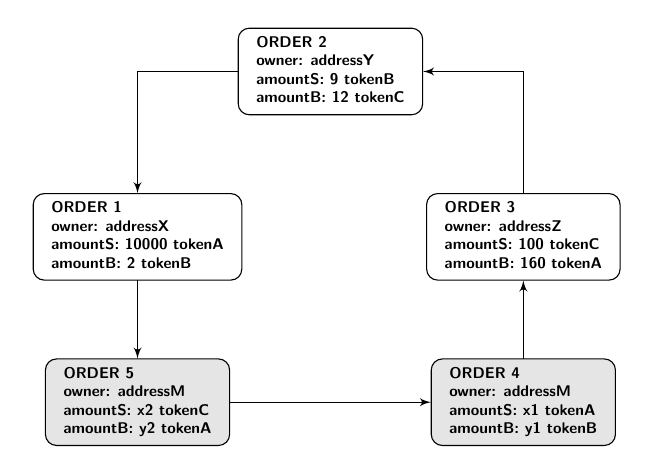
\begin{tikzpicture}[
    auto, 
    node distance=3cm,
    >=latex',
    font=\bfseries\footnotesize\sffamily,
    order/.style={
		scale=0.7,
		rectangle,
		rounded corners,
		draw=black, 
		text centered,
%		text width=5cm,
		minimum height=12mm,
		fill=white
	},
	label/.style={
		scale=0.7
	}
  ]
    % We start by placing the blocks

  \node [order] (order2) 
 {%
 \begin{tabular}{l}
  \textbf{ORDER 2}\\
  \textbf{owner: addressY}\\
  \textbf{amountS: 9  tokenB}\\
  \textbf{amountB: 12 tokenC}
 \end{tabular}
 };
 
  \node [order, below of=order2, xshift=-3.5cm] (order1) 
 {%
 \begin{tabular}{l}
  \textbf{ORDER 1}\\
  \textbf{owner: addressX}\\
  \textbf{amountS: 10000 tokenA}\\
  \textbf{amountB: 2    tokenB}
 \end{tabular}
 };
 
 
  \node [order, below of=order2, xshift=3.5cm] (order3) 
 {%
 \begin{tabular}{l}
  \textbf{ORDER 3}\\
  \textbf{owner: addressZ}\\
  \textbf{amountS: 100   tokenC}\\
  \textbf{amountB: 160 tokenA}
 \end{tabular}
 };
 
   \node [order, below of=order3, fill=gray!20] (order4) 
 {%
 \begin{tabular}{l}
  \textbf{ORDER 4}\\
  \textbf{owner: addressM}\\
  \textbf{amountS: x1 tokenA}\\
  \textbf{amountB: y1 tokenB}
 \end{tabular}
 };
 
 
  \node [order, below of=order1, fill=gray!20] (order5) 
 {%
 \begin{tabular}{l}
  \textbf{ORDER 5}\\
  \textbf{owner: addressM}\\
  \textbf{amountS: x2   tokenC}\\
  \textbf{amountB: y2 tokenA}
 \end{tabular}
 };
 
 \draw [draw,->] (order1) -- node [label, xshift=-2cm] {} (order5);
 \draw [draw,->] (order2) -| node [label, xshift=-1.6cm] {} (order1);
 \draw [draw,->] (order3) |- node [label, xshift=1cm] {} (order2);
 \draw [draw,->] (order4) -- node [label, xshift=1.8cm] {} (order3);
 \draw [draw,->] (order5) -- node [label, yshift=0.2cm] {} (order4);
  
\end{tikzpicture}

\caption{A Ring with Sub-Ring}
\label{fig:ring}
\end{figurehere}
\end{center}

\subsubsection{Fill Rate Checking\label{sec:fill_rate_check}}
The exchange rate calculations in the ring are made by miners for reasons stated above. It is the LSC that must verify they're correct. First, it verifies that the buy rate the miner can execute for each order is equal to or less than the original buy rate set by the user. This ensures the user gets at least the exchange rate they asked for or better on the transaction. Once the exchange rates are confirmed, the LSC ensures that each order in the ring shares the same rate (margin) discount. For instance, if the discounted rate is $\gamma$, then the price for each order will be:

$r_{0\rightarrow 1} \cdot (1-\gamma)$, $r_{1\rightarrow 2} \cdot (1-\gamma)$, $r_{2 \rightarrow 0} \cdot (1-\gamma)$, and satisfied: 
\begin{equation}
r_{0\rightarrow 1} \cdot (1-\gamma)\cdot r_{1\rightarrow 2} \cdot (1-\gamma) \cdot r_{2 \rightarrow 0} \cdot (1-\gamma) = 1
\end{equation}
We can find out: 
\begin{equation*}
\gamma = 1- \frac{1}{\sqrt[3]{r_{0\rightarrow 1} \cdot r_{1\rightarrow 2} \cdot r_{2\rightarrow 0}}}\text{.}
\end{equation*}
If the transaction crosses $n$ orders, the \texttt{discount} is: 
\begin{equation*}
\gamma = 1- \frac{1}{\sqrt[n]{\prod_{i=0}^{n-1} r^i}} \text{,}
\end{equation*}

where $r^i$ is the order turnover rate of $i$-th order. Obviously, only when the discount rate is $\gamma \ge 0$, can these orders be filled; and the $i$-th order's $O^i$ actual exchange rate $\hat{r^i} = r^i \cdot (1-\gamma)$, $\hat{r^i}\le r^i$.

\subsubsection{Fill Tracking \& Cancellation}
A user can partially or fully cancel an order by sending a special transaction to the LSC, containing the details about the order and the amounts to cancel. The LSC takes that into account, stores the amounts to cancel, and emits an $OrderCancelled$ event to the network. The LSC keeps track of fill and cancellation amounts by storing their values using the order's hash as an identifier. This data is publicly accessible and $OrderCancelled$ / $OrderFilled$ events are emitted when it changes. Tracking these values is critical for the LSC during the ring settlement step.


\subsubsection{Order Scaling\label{sec:order_scaling}}
Orders are scaled according to the history of filled and cancelled amounts and the current balance of the senders' accounts. The process finds the order with the smallest amount to be filled according to the above characteristics and uses it as a reference for scaling all transactions in the ring.


Finding the lowest value order can help to figure out the fill volume for each order. For instance, if the $i$-th order is the lowest value order, then the number of tokens sold from each order $\hat{s}$ and number of tokens purchased $\hat{b}$ from each order can be calculated as:

\[
\begin{split}
&\hat{s}^{i}=\overline{s}_i\text{, } \hat{b}^{i}=\hat{s}^{i}/ \hat{r}^i\text{, }\text{;}\\
&\hat{s}^{i\oplus 1}=\hat{b}^i\text{, } \hat{b}^{i\oplus 1}=\hat{s}^{i\oplus 1}/ \hat{r}^{i\oplus 1}\text{;}\\
&\hat{s}^{i\oplus 2}=\hat{b}^{i\oplus 1}\text{, } \hat{b}^{i\oplus 2}=\hat{s}^{i\oplus 2}/ \hat{r}^{i\oplus 2}\text{;}\\
& ...
%\text{.}
\end{split}
\]
where $\overline{s}_i$ is the the balance left after orders are partially filled.

During implementation we can safely assume any order in the ring to have the lowest value, then iterate through the ring at most twice to calculate each order's fill volume. 

Example: If the smallest amount to be filled compared to the original order is 5\%, all the transactions in the ring are scaled down to 5\%. Once the transactions are completed, the order that was considered to have the smallest amount remaining to be filled should be completely filled.

\subsection{Ring Settlement\label{sec:settlement}}

If the Order Ring fulfills all the previous checks, the ring can be closed, and transactions can be made. This means that all the $n$ orders $O$ form a closed ring of orders, connected as in the figure below:

\begin{center}
\begin{figurehere}
\centering
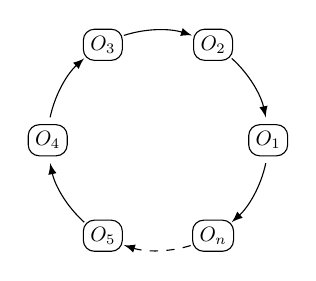
\begin{tikzpicture}[
circle/.style={
		scale=0.75,
		rounded corners,
		draw=black, 
		text centered,
		}
]

\def \n {6}
\def \m {4}
\def \radius {1.4cm}
\def \margin {12} % margin in angles, depends on the radius

\foreach \s in {1,...,\m}
{
  \node[draw, circle] at ({360/\n * (\s - 1)}:\radius) {$O_\s$};
  \draw[<-, >=latex] ({360/\n * (\s - 1)+\margin}:\radius) 
    arc ({360/\n * (\s - 1)+\margin}:{360/\n * (\s)-\margin}:\radius);
}

\node[draw, circle] at ({360/\n * 4}:\radius) {$O_5$};
  \draw[<-, dashed, >=latex] ({360/\n * 4+\margin}:\radius) 
    arc ({360/\n * 4+\margin}:{360/\n * (5)-\margin}:\radius);
    
\node[draw, circle] at ({360/\n * 5}:\radius) {$O_n$};
  \draw[<-, >=latex] ({360/\n * 5+\margin}:\radius) 
    arc ({360/\n * 5+\margin}:{360/\n * (6)-\margin}:\radius);


\end{tikzpicture}
\caption{Ring Settlement}
\label{fig:settlement}
\end{figurehere}
\end{center}

To make the transactions, the LSC uses the $TokenTransferDelegate$ smart contract. The introduction of such a delegate makes upgrading the protocol smart contract easier as all orders only need to authorize this delegate instead of different versions of the protocol.

For each order in the ring, a payment of $tokenS$ is made to the following order. Then the miner's fee is paid depending on the fee model chosen by the miner. An $OrderFilled$ event is then emitted. Finally, once all the transactions are made, a $RingMined$ event is emitted.

\subsubsection{Emitted Events\label{sec:events}}

The protocol emits events that allow relays, order browsers, and other actors to receive order book updates as efficiently as possible. The emitted events are:

\begin{itemize}
	\item \textbf{OrderCancelled}: a specific order has been cancelled.
	\item \textbf{OrdersCancelled}: all orders of a trading pair from an owning address have been cancelled.
	\item \textbf{AllOrdersCancelled}: all orders of all trading pairs from an owning address have been cancelled.
	\item \textbf{RingMined}: A ring has been settled successfully. This event contains data related to each inner-ring token transfer.
\end{itemize}


\section{LRx Token\label{sec:token}}
LRx is our generalized token notation. LRC is the Loopring token on Ethereum, LRQ on Qtum, and LRN on NEO. Other LRx types will be introduced in the future as Loopring is deployed on other public blockchains.

\subsection{Fee Model\label{sec:fee_model}} 
When a user creates an order, they specify an amount of LRx to be paid to the miner as a fee, in conjunction with a percentage of the margin made on the order that the miner can claim. This is called the margin split. The decision of which one to choose is left to the miner.

A representation of the margin split:

\begin{center}
\begin{figurehere}
\centering
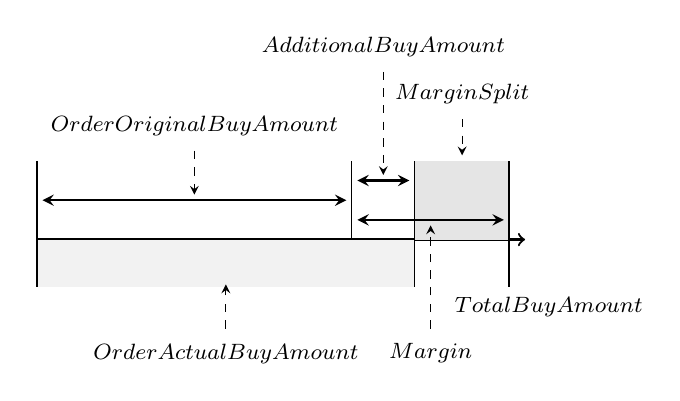
\begin{tikzpicture}[
scale=1,
font=\bfseries\footnotesize\sffamily,
classical/.style={thick,<->,shorten >=2pt,shorten <=2pt,>=stealth},
oneway/.style={->,dashed,shorten >=2pt,shorten <=2pt,>=stealth}
]
    % Draw axes
    \draw [->,thick] (0,1) node (yaxis) [above] {$$}
        |- (6.2,0) node (xaxis) [right] {$$};
        
    \draw
  	(4,0) coordinate (A)
  	(4,1) coordinate (A2)
  	(4.8,-0.6) coordinate (B)
  	(4.8,1) coordinate (B2)
  	(6,-0.6) coordinate (C)
  	(6,1) coordinate (C2);
  	
  	\fill [draw=none, fill=gray!20] 
    (4.8, 0) rectangle (6, 1);
    
  	\fill [draw=none, fill=gray!10] 
    (0, -0.6) rectangle (4.8, 0);

	\draw[thick] (0, -0.6) -- (0, 0.6) node[below]{$$};
  	\draw[thick, thin] (A) -- (A2) node[below]{$$};
  	\draw[thick, thin] (B) -- (B2) node[below]{$$};
  	\draw[thick] (C) node[below, xshift=0.5cm]{$Total Buy Amount$} -- (C2) ;
  	
  	\draw[classical] (0, 0.5) -> (4, 0.5) node[below]{$$};
  	\draw[classical] (4, 0.75) -> (4.8, 0.75) node[below]{$$};
%  	\draw[classical] (4.8, 0.5) -> (6, 0.5) node[below]{$$};
  	\draw[classical] (4, 0.25) -> (6, 0.25) node[below]{$$};

  	
  	\draw[oneway] (2, 1.2) node[above]{$Order Original Buy Amount$} -- (2, 0.5);
  	\draw[oneway] (4.4, 2.2) node[above]{$Additional Buy Amount$} -- (4.4, 0.75);
  	\draw[oneway] (5.4, 1.6) node[above]{$Margin Split$} -- (5.4, 1);
  	\draw[oneway] (5, -1.2) node[below]{$Margin$} -- (5, 0.25);
  	\draw[oneway] (2.4, -1.2) node[below]{$Order Actual Buy Amount$} -- (2.4, -0.5);



\end{tikzpicture}
\caption{A 60\% Margin Split}
\label{fig:marginsplit}
\end{figurehere}
\end{center}

If the margin on the ring is too small, a miner will choose the LRx fee. If, on the contrary, the margin is substantial enough for the resulting margin split to be worth more than the LRx fee, a miner will choose the margin split. There is another proviso, however: when the miner chooses the margin split, they must pay the user (order creator) a fee, which is equal to the LRx the user would have paid to the miner as a fee. This increases the threshold of where the miner will choose the margin split to twice the LRx fee of the order, increasing the propensity of the LRx fee choice. This allows miners to receive a constant income on low margin rings for the tradeoff of receiving less income on higher margin rings. Our fee model is based on the expectation that as the market grows and matures, there will be fewer high margin rings, thus necessitating fixed LRx fees as incentive.


We end up with the following graph:

\begin{center}
\begin{figurehere}
\centering
\begin{tikzpicture}[
font=\bfseries\footnotesize\sffamily,
scale=1.5]
    % Draw axes
    \draw [<->,thick] (0,2.8) node (yaxis) [above] {$y$}
        |- (4,0) node (xaxis) [right] {$x$};
        
    \draw
  	(1,1) coordinate (A)
  	(2,1) coordinate (B);
  	
  	
  	\draw[thick] (B) -- (3.7,2.7);
  	\draw[dotted] (B) -- (2,0) node[below] {$2f$};
  	\draw[dotted] (A) -- (1,0) node[below] {$f$};
  	\draw[dashed] (0,0) -- (2.7,2.7);
  	\draw[thick] (0,1) node[left] {$f$}--(B) node[
      circle,
      draw,
      fill=white,
      inner sep = 1pt,
      minimum size = 4pt,
     ]{$$};



\end{tikzpicture}
\caption{Loopring Fee Model}
\label{fig:feemodel}
\end{figurehere}
\end{center}

where $f$ is the LRx fee, $x$ is the margin split, $y$ is the mining income. $y=max(f, x-f)$ as indicated by the solid line; if the LRx fee for the order is $0$, the equation is $y=max(0, x - 0)$ that simplifies to $y=x$ as indicated by the dashed line.\\

The consequences are:  
\begin{enumerate}
	\item If the margin split is 0, the miners will choose the flat LRx fee and are still incentivized. 
	\item If the LRx fee is 0, the orange line results and the income is based on a general linear model.
	\item When the margin split income is greater than 2x(LRx fee), the miner chooses the margin split.
\end{enumerate}

It should be noted that if the LRx fee is non-zero, no matter which option the miner chooses, there will always be a transfer of LRx between the miner and the order's sender. Either the miner earns the LRx fee, or pays the LRx fee back to the sender to take the margin split.

Ring miners will share a certain percentage of fees with wallets. When a user places an order through a wallet and gets filled, the wallet is rewarded with a portion of the fees or margin split. Wallets represent a primary target for Loopring protocol integration as they have the user base, but little source of income.

\subsection{Decentralized Governance}
At its root, the Loopring protocol is a social protocol in the sense that it relies on coordination amongst members to operate effectively towards a goal. This is not dissimilar to cryptoeconomic protocols at large, and indeed, its usefulness is largely protected by the same mechanisms of coordination problems \cite{vitalikgovernance}, grim trigger equilibrium, and bounded rationality. To this end, LRx tokens are not only used to pay fees, but also to align the financial incentives of the various network participants. Such alignment is necessary for broad adoption of any protocol, but is particularly acute for exchange protocols, given that success rests largely on improving liquidity in a robust decentralized ecosystem.

LRx tokens will be used to effectuate protocol updates through decentralized governance. Smart contract updates will be governed by token holders to ensure continuity and safety, and to attenuate the risks of siphoned liquidity through incompatibility. Given that smart contracts cannot be altered once deployed, there is a risk that dApps or end users continue to interact with deprecated versions and preclude themselves from updated contracts. Upgradeability is crucial to the protocol's success as it must adapt to market demands and the underlying blockchains. Decentralized governance by LRx stakeholders will allow for protocol smart contract updates without disrupting dApps or end users. At first, this will be done through a simple multisignature smart contract.

\section{Fraud and Attack Protections}

\subsection{Front-running Prevention\label{sec:dual_authoring}}

In decentralized exchanges, front-running is when someone tries to copy another node's ring solution, and have it mined before the original transaction that is in the pending transaction pool (mempool). This can be achieved by specifying a higher transaction fee (gas price). The major scheme of front-running in Loopring (and any protocol for order-matching) are order-filch: when a front-runner steals one or more orders from a pending ring settlement transaction; and Ring-filch: when a front-runner steals the entire ring from the pending transaction.

When a submitRing transaction is not confirmed and still in the pending transaction pool, anyone can easily spot such a transaction and replace $miner\_address$ with their own address (the filcher\_address) , then they can re-sign the payload with filcher\_address to replace the ring's signature. The fincher can set a higher gas price and submit a new transaction hoping block miners will pick his new transaction into the next block instead of the original submitRing transaction.

Previous solutions to this problem had important downsides (v1.1): requiring more transactions and thus cost miners more gas; and taking at least twice the blocks to settle a ring.  Our new solution involves the mechanism of setting up two levels of authorization for orders - one for settlement, and one for mining.

How it works:

\begin{enumerate}

	\item For each order, the wallet software will generate a random public-key/private-key pair, and put the key pair into the order's JSON snippet. (An alternative is to use the address derived from the public-key instead of the public-key itself to reduce byte size. We use $authAddr$ to represent such an address, and $authKey$ to represent $authAddr$'s matching private-key).

	\item All fields in the order except $authKey$ is signed using the $owner$ address's private-key (not $authKey$) as shown in the image below.

	\item The wallet will send the order, together with the $authKey$ to miners (relays) for matching.The miner will verify that $authKey$ and $authAddr$ are correctly paired and the order's signature is valid with respect to owner\_address.

	\item When a ring is identified, the miner will use each order's $authKey$ to sign the ring's hash, $miner\_address$, and all the mining parameters. In the example below, the ring contains 3 orders, therefore there will be 3 signatures by the 3 $authKey$s. We call these signatures the $auth\_signature$s. The miner also needs to sign the ring's hash together with all mining parameters using $miner\_address$'s private-key.

	\item The miner calls the submitRing function with all the parameters, as well as the 3 extra $auth\_signature$s. Notice that $authKey$s are NOT part of the on-chain transaction and thus remain unknown to people other than the relay itself, as shown in the image below.

	\item The Loopring Protocol will now verify each $auth\_signature$ against the corresponding $authAddr$ of each order, and reject the ring if any $auth\_signature$ is invalid.
 
\end{enumerate}
[TODO: daniel wang]


The result is that now:

\begin{itemize}

	\item  The order’s signature (by the private-key of the $owner\_address$) guarantees the order cannot be modified, including the $authAddr$.
	\item  The miner’s signature (by the private-key of the $miner\_address$) guarantees nobody can use his identity to mine a ring.
	\item  The $auth\_signature$s guarantees the entire ring cannot be modified, including $miner\_address$. And since ring-filchers do not have access to $authKey$s, they cannot re-generate a new set of $auth\_signature$s thus are unable to generate a filch transaction.

\end{itemize}

Dual Authoring prevents ring-filch and order-filch while still ensuring the settlement of rings can be done in one single transaction. In addition, Dual Authoring opens doors for relays to share orders in two ways: non-matchable sharing and matchable sharing. Loopring operates an OTC model and only supports limit-price orders, meaning that orders’ timestamps are totally ignored. This implies that front-running a trade has no impact on the actual price of that trade, but does impact whether it gets filled or not.

\section{Other Attacks}

\subsection{Sybil or DOS Attack}
Malicious users - acting as themselves or forged identities - could send a large amount of small orders to attack Loopring nodes. However, since we allow nodes to reject orders based on their own criteria - which they may hide or reveal - most of these orders will be rejected bfor not yielding satisfying profit when matched.  By empowering relayers to dictate how they manage orders, we do not see a massive tiny order attack as a form of unethical behaviour.

\subsection{Insufficient Balance}
Malicious users could sign and spread orders whose value inside the order is non-zero but whose address actually has zero balance. Nodes could monitor and notice that some orders actual balance is zero, update these order states accordingly and then discard them.
Nodes must spend time to update the status of an order, but can also choose to minimize the effort by, for example, blacklisting addresses and dropping related orders.

\section{Summary}
The Loopring protocol sets out to be a foundational layer for decentralized exchange. In so doing, it has profound repurcussions in how people exchange assets and value. Money, as an intermediate commodity, facilitates or replaces barter exchange and solves the double coincidence of wants problem \cite{unenumerated2006}, whereby two counterparties must desire each other's distinct good or service. Similarly, Loopring protocol aims to dispense of our dependencies on coincidence of wants in trading pairs by using ring matching to more easily consummate trades. This is meaningful for how society and markets transfer value with tokens, traditional assets, and beyond. Indeed, just as decentralized cryptocurrencies pose threat to a nation's control over money, a combinatorial algorithm that can match traders (consumers/producers) at scale, is a threat to the concept of money itself. In addition, with Dual Authoring, Loopring solves the real and pernicious problem of front running faced by all decentralized exchanges and their users today.

\begin{itemize}
	\item Off-chain order management and on-chain settlement = no sacrifice in performance for security.
	\item Network maintained by self-motivated group of relays with flexibility in running order books and communicating.
	\item Greater liquidity due to more counterparties available through order sharing, and higher probability that any counterparty can be a useful trading partner due to multi-party trades.
	\item Free, public smart contracts enable any dApp to build or interact with the protocol.
	\item Standardization among operators allows for network effects, deeper liquidity and an improved end user experience.
	\item Reduced barriers to entry for market-makers = lower costs for nodes joining the network and end users.
	\item Anonymous trading directly from users’ wallets.
\end{itemize}

\section{Acknowledgements}
We would like to express our gratitude to our mentors, advisers and to the many people in the community that have been so welcoming and generous with their knowledge. In particular, we would like to thank Shuo Bai (from ChinaLedger); Professor Haibin Kan; Alex Cheng, Hongfei Da; Yin Cao; Xiaochuan Wu; Zhen Wang, Wei Yu, Nian Duan, Jun Xiao, Jiang Qian, Jiangxu Xiang, Yipeng Guo, Dahai Li, Kelvin Long, Huaxia Xia, Jun Ma, and Encephalo Path for reviewing and providing feedback on this project. We welcome more feedback from the community.



\bibliography{whitepaper2}
\bibliographystyle{unsrt}


\end{multicols}

\newpage











\begin{figure}[h]
\centering
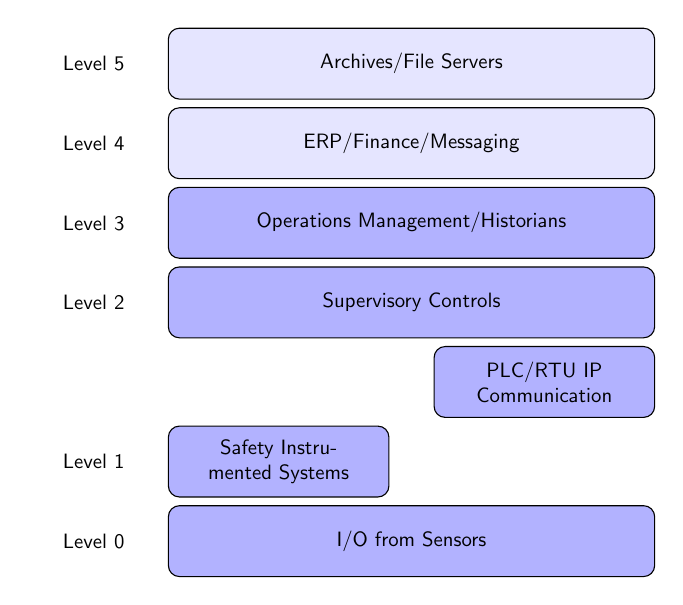
\begin{tikzpicture}[
	scale=0.75,
	start chain=1 going below, 
	start chain=2 going right,
	node distance=1mm,
	desc/.style={
		scale=0.75,
		on chain=2,
		rectangle,
		rounded corners,
		draw=black, 
		text centered,
		text width=8cm,
		minimum height=12mm,
		fill=blue!30
		},
	it/.style={
		fill=blue!10
	},
	level/.style={
		scale=0.75,
		on chain=1,
		minimum height=12mm,
		text width=2cm,
		text centered
	},
	every node/.style={font=\sffamily}
]

% Levels
\node [level] (Level 5) {Level 5};
\node [level] (Level 4) {Level 4};
\node [level] (Level 3) {Level 3};
\node [level] (Level 2) {Level 2};
\node [level] (Level 1.5) { };
\node [level] (Level 1) {Level 1};
\node [level] (Level 0) {Level 0};

% Descriptions
\chainin (Level 5); % Start right of Level 5
% IT levels
\node [desc, it] (Archives) {Archives/File Servers};
\node [desc, it, continue chain=going below] (ERP) {ERP/Finance/Messaging};
% ICS levels
\node [desc] (Operations) {Operations Management/Historians};
\node [desc] (Supervisory) {Supervisory Controls};
\node [desc, text width=3.5cm, xshift=2.25cm] (PLC) {PLC/RTU IP Communication};
\node [desc, text width=3.5cm, xshift=-4.5cm] (SIS) {Safety Instrumented Systems};
\node [desc, xshift=2.25cm] (IO) {I/O from Sensors};

\end{tikzpicture}
\caption{FOSS in Chrome influences industry structure by increasing competition}
\label{fig:6forces}
\end{figure}




































\begin{appendices}

\section{Protocol Ethereum Smart-Contracts\label{app:protocol_ethereum}}



\begin{center}
\begin{figurehere}
\centering
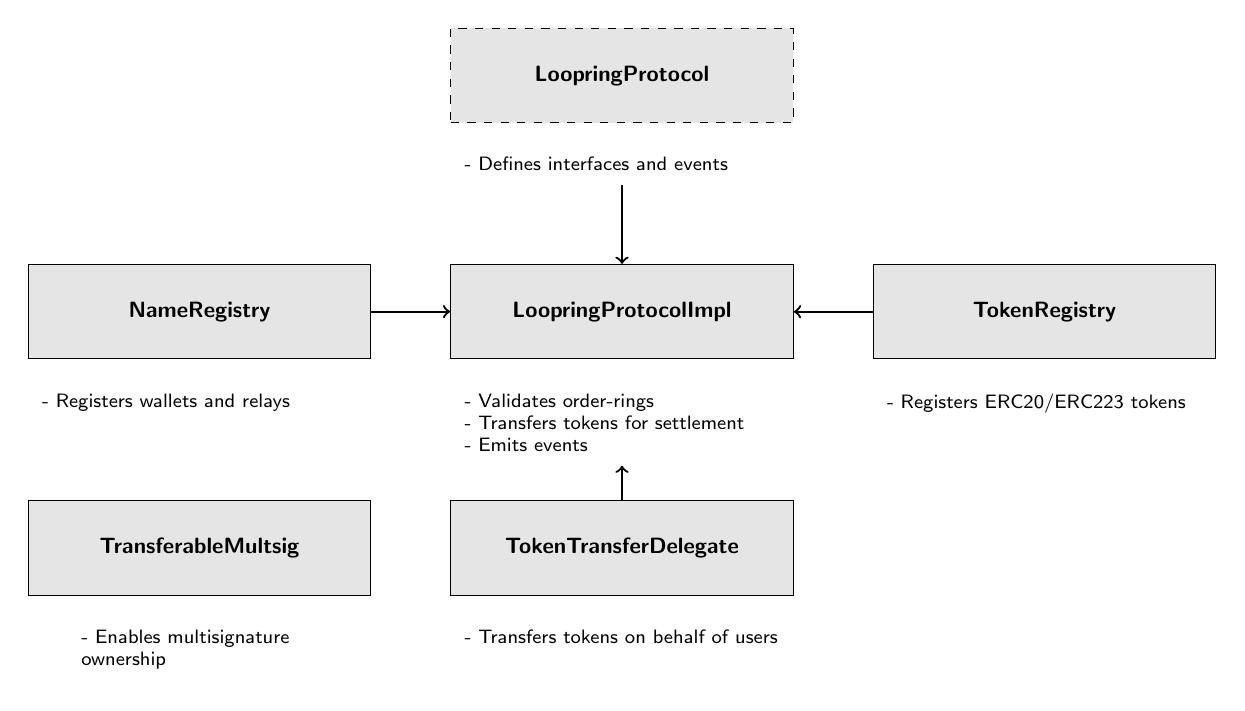
\begin{tikzpicture}
[node distance = 1cm, auto,font=\footnotesize,
% STYLES
every node/.style={node distance=3cm},
% The comment style is used to describe the characteristics of each force
comment/.style={rectangle, inner sep= 5pt, text width=4cm, node distance=0.25cm, font=\scriptsize\sffamily},
% The force style is used to draw the forces' name
force/.style={rectangle, draw, fill=black!10, inner sep=5pt, text width=4cm, text badly centered, minimum height=1.2cm, font=\bfseries\footnotesize\sffamily}] 

% Draw forces
\node [force] (impl) {LoopringProtocolImpl};
\node [force, dashed, above of=impl] (protocol_interface) {LoopringProtocol};
\node [force, left=1cm of impl] (nameregistry) {NameRegistry};
\node [force, right=1cm of impl] (tokenregistry) {TokenRegistry};
\node [force, below of=impl] (delegate) {TokenTransferDelegate};
\node [force, left=1cm of delegate] (multisig) {TransferableMultsig};

%%%%%%%%%%%%%%%
% Change data from here

% impl
\node [comment, below=0.25 of impl] (comment-impl) {- Validates order-rings\\
- Transfers tokens for settlement\\
- Emits events};

% nameregistry
\node [comment, below=0.25cm of nameregistry]{- Registers wallets and relays};

% protocol_interface
\node [comment, below=0.25 of protocol_interface](comment-interface) {- Defines interfaces and events};

% tokenregistry
\node [comment, below=0.25 of tokenregistry] {- Registers ERC20/ERC223 tokens};

% delegate
\node [comment, below=0.25 of delegate] {- Transfers tokens on behalf of users};

% PUBLIC POLICIES
\node [comment, text width=3cm, below=0.25 of multisig] {- Enables multisignature ownership};

%%%%%%%%%%%%%%%%

% Draw the links between forces
\path[->,thick] 
(comment-interface) edge (impl)
(nameregistry) edge (impl)
(tokenregistry) edge (impl)
(delegate) edge (comment-impl);

\end{tikzpicture} 
\caption{Loopring Ethereum Smart-Contracts}
\label{fig:smartcontracts}
\end{figurehere}
\end{center}

The source code of these smart contract are available at:\\
https://github.com/Loopring/protocol/tree/master/contracts.


\end{appendices}
\end{document}
